\documentclass{article}
\usepackage{fancyhdr}
\usepackage{amsmath}
\usepackage{titlesec}
\usepackage{amsfonts}
\usepackage{graphicx}

\titleformat*{\section}{\large\bfseries}
\titleformat*{\subparagraph}{\bfseries}

\pagestyle{empty}
\fancyhf{}
\cfoot{\thepage}

\lhead{Stephanie Slayden\\David Vejvalka\\Mihai Dobri}
\rhead{
CIS 761 \\
Database Design}

\begin{document}

\setlength{\headheight}{30pt}
\thispagestyle{fancy}
$ $ \\
\textbf{Application domain, desired functionality and constraints:} \\ \\
Our database represents an online movie rental store. The store will have customers. Each customer has a customer id, which is the key, a first name, a last name, a phone number, and a birthday. The birthday will determine what customers are able to rent what movies based on their rating. The store will also have rentals. A rental consists of a rental id (the key), a movie id, a customer id, and the day the rental was placed. We will also have a movie table. This table will store information about the movie. We will have a movie id (the key), the movie title, the year the movie was released, the price to rent the movie, the producer and the rating. We will have a producer table which will have a producer id and the name of the producer. We are assuming that there will only be one prodcer per movie. A movie can have multiple genres, thus we will have a genre table with the movie id and the name of the genre. We will also have an actor table. This will have an actor id, first name, and last name. This will be an online rental store similar to how movies can be rented from Amazon. Each rental will expire after 30 days.

\section*{(a)}
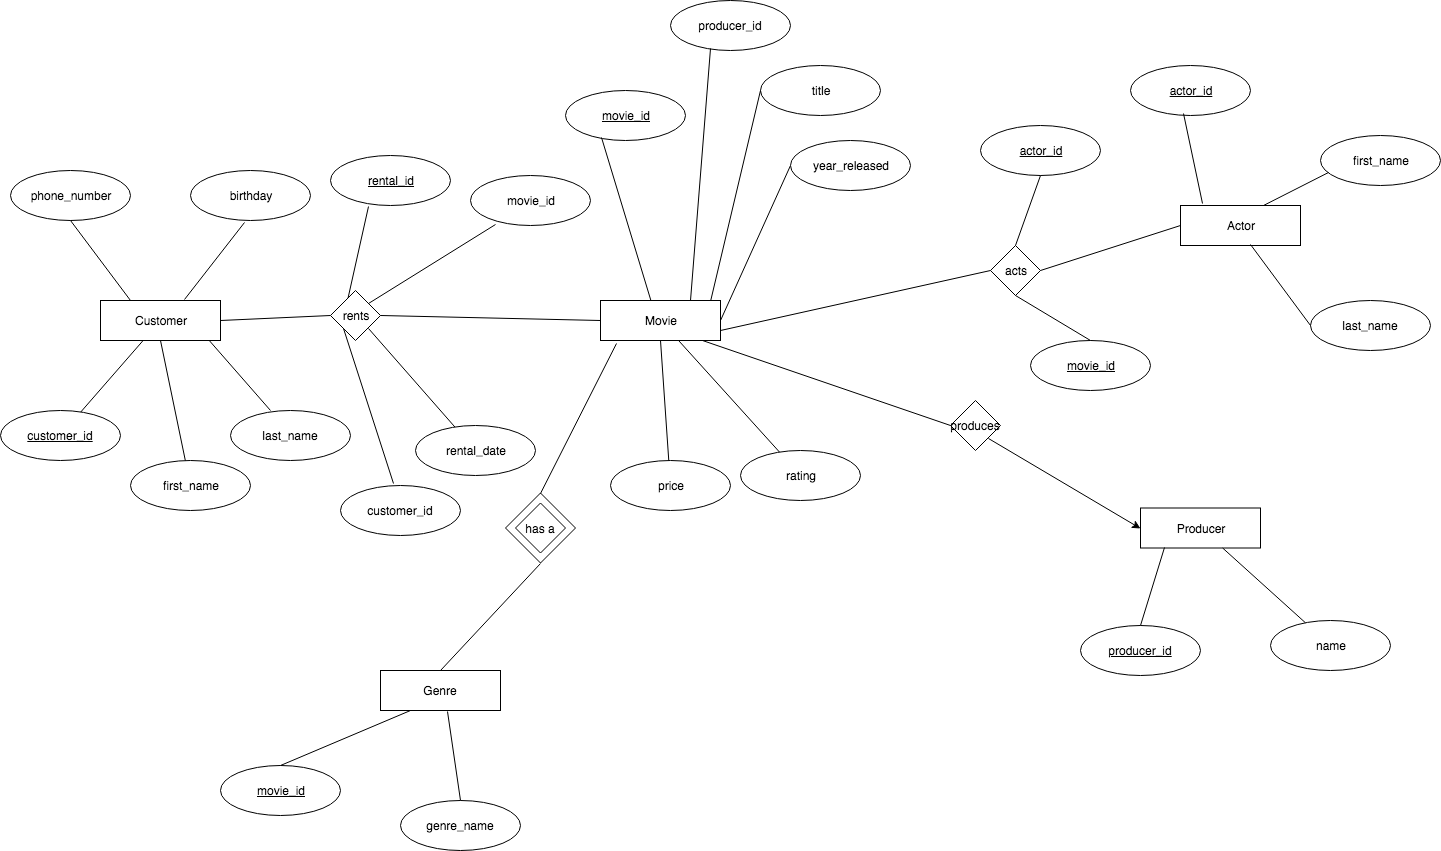
\includegraphics[scale = 0.3]{moviedb.png}

\section*{(b)}
$ $ \\
Customer(\underline{customer\_id}, first\_name, last\_name, phone\_number, birthday) \\
Rental(\underline{rental\_id}, movie\_id, customer\_id, rental\_date) \\
Movie(\underline{movie\_id}, producer\_id, title, year\_released, rating, price) \\
Producer(\underline{producer\_id}, name) \\
Actor(\underline{actor\_id}, first\_name, last\_name) \\
Actor\_Movie(\underline{actor\_id}, \underline{movie\_id}) \\
Genre(\underline{movie\_id}, genre\_name)

\section*{(c)}
None of our relations have any nonrivial functional dependencies. It could be argued that in the `Customer' relation the phone number is unique and could determine the other attirbutes. However, we do not believe this to be true in our model, as a child could possibly share the same number as their parents or a specific phone number could be disconnected and then used again for another customer. Thus, we have no nontrivial functional dependencies.

\section*{(d)}
As stated above, we do not have any nontrivial functional dependencies. Thus our schema is in BCNF.

\end{document}